\chapter{Implementasi dan Pengujian}
\label{chap:implementasidanpengujian}

Bab ini membahas mengenai implementasi dan pengujian perangkat lunak SharIF Judge.

\section{Lingkungan Implementasi dan Pengujian}
\label{sec:5:lingkungan}

Implementasi perangkat lunak dilakukan pada beberapa lingkungan yang berbeda:

\begin{itemize}
    \item Lingkungan \textit{development}: \\ Perangkat lokal milik penulis yang digunakan untuk pembangunan perangkat lunak. Spesifikasi lingkungan ini adalah sebagai berikut:
    \begin{itemize}
        \item Perangkat Keras:
        \begin{itemize}
            \item \textit{Processor}: Intel Core i5-7600 3.5GHz
            \item \textit{Random Access Memory}: 16GB DDR4
            \item \textit{Storage}: 500GB
        \end{itemize}
            \item Perangkat Lunak:
        \begin{itemize}
            \item \textit{Operating System}: Windows 10 Home 64-bit
            \item \textit{Windows Subsystem for Linux}: Ubuntu 20.04.2 LTS
        \end{itemize}
    \end{itemize}
    
    \item Lingkungan \textit{staging}: \\ Lingkungan \textit{server} yang digunakan untuk menguji perangkat lunak selama pembangunan. Spesifikasi lingkungan ini adalah sebagai berikut:
    \begin{itemize}
    \item Perangkat Keras:
        \begin{itemize}
            \item \textit{Processor}: Intel DO-Regular 2.4GHz
            \item \textit{Random Access Memory}: 1GB
            \item \textit{Storage}: 25GB
        \end{itemize}
            \item Perangkat Lunak:
        \begin{itemize}
            \item \textit{Operating System}: Ubuntu 20.04.3 LTS
        \end{itemize}
    \end{itemize}
    
    \item Lingkungan \textit{production}: \\ Lingkungan \textit{server} yang digunakan pada kuliah Dasar-dasar Pemrograman dengan alamat \verb|http://daspro.labftis.net|. Spesifikasi lingkungan ini adalah sebagai berikut:
    \begin{itemize}
    \item Perangkat Keras:
        \begin{itemize}
            \item \textit{Processor}: Intel Xeon E5-2603 1.70GHz
            \item \textit{Random Access Memory}: 8GB
            \item \textit{Storage}: 1TB
        \end{itemize}
            \item Perangkat Lunak:
        \begin{itemize}
            \item \textit{Operating System}: Ubuntu 16.04.6 LTS
        \end{itemize}
    \end{itemize}
\end{itemize}

\section{Implementasi}
\label{sec:5:implementasi}

\subsection{Tampilan Antarmuka}
\label{subsec:5:antarmuka}

\begin{figure}[H]
	\centering  
	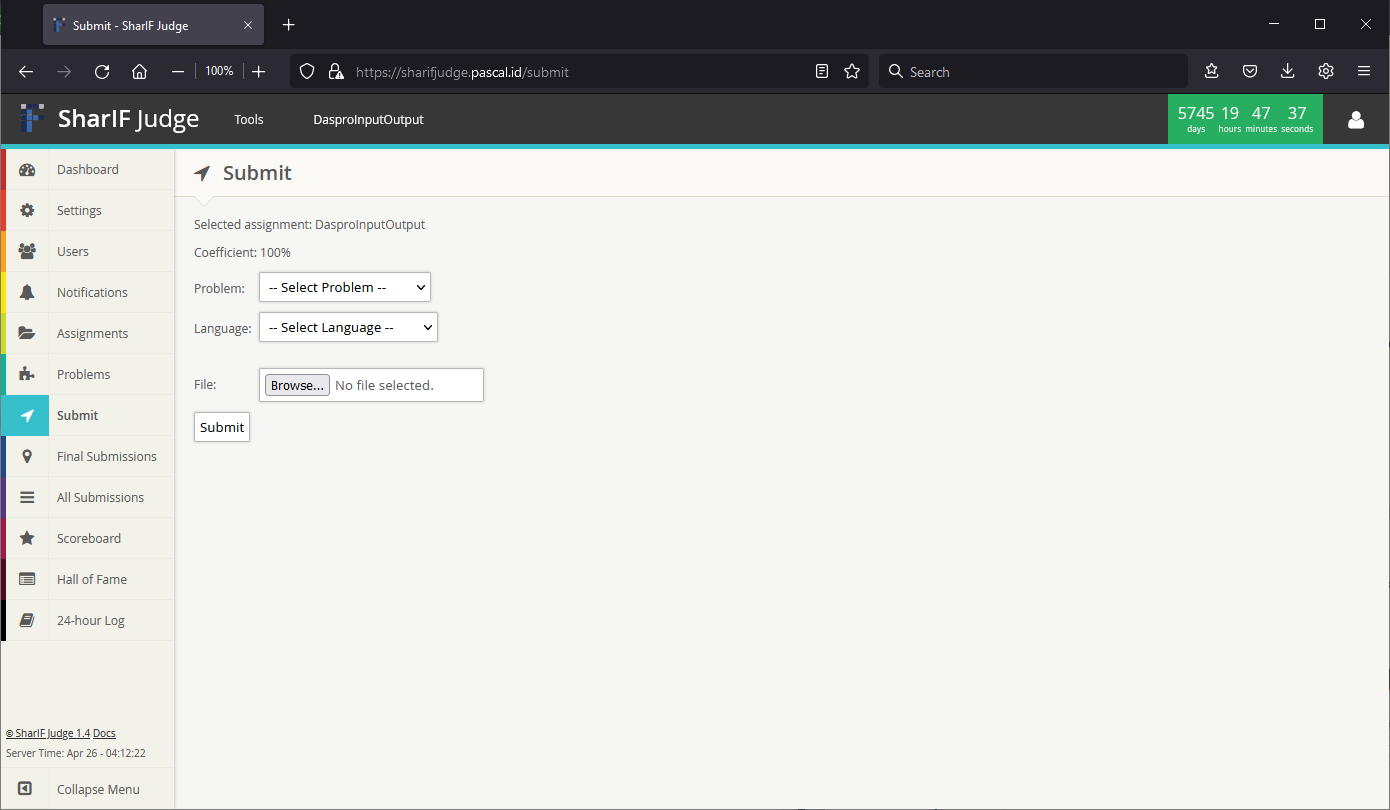
\includegraphics[scale=0.3]{submit}  
	\caption{Antarmuka halaman Submit} 
	\label{fig:5:antarmuka} 
\end{figure}

Gambar \ref{fig:5:antarmuka} merupakan tampilan antarmuka pada halaman Submit yang sudah diimplementasikan. Seluruh perubahan pada \verb|submit.twig| dapat dilihat pada lampiran \ref{lampA:Submit.twig}. Seluruh \textit{style} dan \textit{script} untuk halaman ini terletak di \textit{file} terpisah. \textit{Stylesheet} yang terdapat di \verb|assets\styles\submit.css| dapat dilihat pada lampiran \ref{lampA:submit.css}. \textit{Script} yang terdapat di \verb|assets\js\shj_submit.js| dapat dilihat pada lampiran \ref{lampA:shj_submit.js}.

\subsection{Menampilkan Soal}
\label{subsec:5:soal}

Soal PDF ditampilkan pada \verb|iframe| yang berisi \verb|viewer.html| milik PDF.js. URL dari \textit{file} PDF yang akan ditampilkan adalah URL yang mengarah ke fungsi \verb|pdf| pada controller \verb|Assignments|. URL ini dikirim ke \verb|viewer.html| PDF.js sebagai parameter GET bernama \verb|site_url|.

Fungsi \verb|pdf| pada controller \verb|Assignments| menggunakan fungsi \verb|force_download| yang menyebabkan munculnya dialog unduh pada \textit{browser}. Agar \textit{file} PDF dapat dibaca oleh \textit{browser} dan tidak memunculkan dialog unduh, \textit{file} PDF akan dikembalikan dengan fungsi \verb|die| dengan header \verb|Content-Type: application/pdf|. Ditambahkan parameter \verb|$no_download| pada fungsi \verb|pdf| untuk menentukan apakah \textit{file} PDF soal akan diunduh atau ditampilkan oleh PDF.js. Jika \verb|$no_download| bernilai \verb|FALSE|, maka PDF akan diunduh melalui fungsi \verb|force_download| seperti semula. Jika \verb|$no_download| bernilai \verb|TRUE|, maka PDF akan dikembalikan melalui fungsi \verb|die|. Kode untuk perubahan ini dapat dilihat pada lampiran \ref{lampA:Assignments.php}

\subsection{Editor Kode}
\label{subsec:5:editor}

Ace menggunakan sebuah elemen \verb|div| sebagai tempat untuk menampilkan editor kodenya. Editor ace dimuat dan dikonfigurasi melalui JavaScript yang terdapat di \verb|shj_submit.js|. Ditambahkan juga beberapa fungsi untuk mengubah konfigurasi \textit{syntax highlighting} sesuai dengan bahasa yang dipilih, dan untuk mengaktifkan atau menonaktifkan editor kode jika \textit{problem} dan bahasa belum dipilih. Kode JavaScript untuk konfigurasi editor Ace dapat dilihat pada lampiran \ref{lampA:shj_submit.js}.

\subsection{Menyimpan dan Memuat Kode}
\label{subsec:5:simpan}

Kode akan disimpan pada \textit{file} txt bernama \verb|editor.txt|. Nama dan tipe file ini disimpan sebagai konstanta pada \verb|constants.php|. Perubahan kode \verb|constants.php| dapat dilihat pada lampiran \ref{lampA:constants.php}.

Untuk menyimpan kode, fungsi \verb|save| ditambahkan pada \textit{controller} \verb|Submit|. Fungsi ini mengambil isi dari editor kode melalui POST lalu menyimpannya pada \verb|editor.txt|. Kode untuk fungsi \verb|save| dapat dilihat pada lampiran \ref{lampA:Submit.php} baris 72--135.

Untuk memuat kode, fungsi \verb|load| ditambahkan pada \textit{controller} \verb|Submit|. Bila tersedia, fungsi ini mengambil isi dari \verb|editor.txt| txt lalu mengembalikan isinya. Kode untuk fungsi \verb|load| dapat dilihat pada lampiran \ref{lampA:Submit.php} baris 39--64.

Fungsi \verb|save| dan \verb|load| dipanggil melalui \textit{AJAX request} pada \verb|shj_submit.js|. Fungsi \verb|save| dipanggil ketika tombol Save ditekan, sementara fungsi \verb|load| dipanggil ketika pengguna memilih \textit{problem} pada \textit{dropdown}. Kode JavaScript untuk mengirimkan \textit{AJAX request} tersebut dapat dilihat pada lampiran \ref{lampA:shj_submit.js} baris 77--99 dan baris 23--47.

\subsection{Menjalankan Kode dengan Tes Kasus}
\label{sec:5:jalan}

Pada sistem antrean kode yang dibahas pada bagian \ref{subsec:3:antrean}, tabel \verb|shj_queue| tidak menyimpan alamat dan ekstensi \textit{file}, namun tabel ini menyimpan \verb|submit_id| sebagai referensi untuk tabel \verb|shj_submissions|, dimana alamat dan ekstensi \textit{file} tersimpan. Selain itu, \verb|submit_id| juga digunakan untuk menyimpan nilai yang dihasilkan oleh \verb|tester.sh|. Karena itu, agar kode dapat dimasukkan pada antrean, kode perlu dikumpulkan sebagai \textit{submission} terlebih dahulu. 

Agar kode dari editor dapat dijalankan melalui antrean yang sama, perlu dilakukan langkah-langkah berikut ini:
\begin{enumerate}
    \item Kode yang sudah disimpan sebagai \textit{file} txt disimpan kembali dengan ekstensi yang tepat.
    \item \textit{Input} tes kasus disimpan sebagai \textit{file} txt.
    \item Membuat \textit{entry} pada tabel \verb|shj_submission| yang bersifat sementara untuk menyimpan alamat dan ekstensi \textit{file} kode. Dikarenakan \verb|submit_id| untuk setiap \textit{submission} selalu dimulai dari 1, \textit{submission} dapat digunakan \verb|submit_id| = 0.
    \item Membuat \textit{entry} pada tabel \verb|Queue| dengan \verb|submit_id| = 0 dan \verb|type = "exec"| untuk menandakan bahwa kode ini bukan \textit{submission} yang akan dinilai.
    \item Ditambahkan parameter dan fungsi pada \verb|tester.sh| yang menjalankan kode dengan tes kasus yang sudah disimpan tanpa melakukan penilaian, lalu menyimpan hasil \textit{output} kode sebagai \textit{file} txt.
    \item \textit{File} txt \textit{output} dimuat dan ditampilkan pada halaman submit.
\end{enumerate}

\textit{Input} dan \textit{output} kode akan disimpan pada \textit{file} txt bernama \verb|exec_in.txt| dan \verb|exec_out.txt|. Nama dan tipe file ini disimpan sebagai konstanta pada \verb|constants.php|. Ditambahkan juga konstanta yang akan digunakan sebagai \verb|submit_id| antrean dari seluruh kode yang akan dijalankan. Perubahan kode \verb|constants.php| dapat dilihat pada lampiran \ref{lampA:constants.php}.

Untuk menyimpan kode, fungsi \verb|_execute| ditambahkan pada \textit{controller} \verb|Submit|. Fungsi ini dijalankan oleh fungsi \verb|save("execute")| setelah \textit{file} berhasil disimpan. Kode disimpan kembali dengan ekstensi yang sesuai, lalu informasinya disimpan melalui \textit{model} \verb|Queue_model|. Perubahan kode ini dapat dilihat pada lampiran \ref{lampA:Submit.php}

\subsubsection{Penamaan File Java}

\subsection{Mengumpulkan Kode dari Editor}
\label{subsec:5:kumpul}

\section{Pengujian}
\label{subsec:5:pengujian}

\subsection{Pengujian Fungsional}
\label{subsec:5:fungsional}

Pengujian fungsional dilakukan secara lokal pada perangkat penulis. Berikut ini pengujian yang dilakukan terhadap fitur-fitur yang sudah diimplementasi:

\begin{table}[H]
	\centering
	\caption{Tabel Pengujian Fungsional}
	\begin{tabular}{|p{0.5cm}| p{5.5cm}| p{6cm}| p{2.5cm}|} \hline
	No.	&	Aksi Pengguna	&	Reaksi yang diharapkan	&	Reaksi Perangkat Lunak \\ \hline
	1 	&  Membuka halaman Submit, dengan \textit{assignment} yang dipilih memiliki PDF soal & PDF Soal ditampilkan &	sesuai	\\ \hline
	2 	&  Memilih \textit{problem} dan \textit{language} pada dropdown & Editor kode dan tombol Save, Submit, Execute diaktifkan &	sesuai	\\ \hline
	3 	&  Mengetik kode pada editor kode & Kode yang diketik memiliki \textit{syntax highlighting} sesuai dengan bahasa yang dipilih &	sesuai	\\ \hline
	4 	&  Menekan tombol save & Kode disimpan ditandai dengan \textit{status} "Saved" &	sesuai	\\ \hline
	5 	&  Memilih \textit{problem} pada dropdown setelah menyimpan kode & Kode dimuat pada editor kode &	sesuai	\\ \hline
	6 	&  Menekan tombol Execute & \textit{Output} kode sesuai dengan tes kasus ditampilkan &	sesuai	\\ \hline
	7 	&  Menekan tombol Submit & Pengguna diarahkan ke halaman All Submissions dengan kode pada editor berhasil dikumpulkan dan dinilai  &	sesuai	\\ \hline
	\end{tabular}
	\label{table:fungsional}
\end{table}


\subsection{Pengujian Eksperimental}
\label{subsec:5:eksperimental}

Pengujian eksperimental dilakukan pada mata kuliah Dasar-dasar Pemrograman semester 51 Teknik Informatika Unpar. Perangkat lunak diuji pada \textit{judge} dengan alamat \verb|http://daspro.labftis.net|. Seluruh persoalan dan masukan yang diterima selama mata kuliah Dasar-dasar Pemrograman dicatat pada \verb|https://github.com/athlonneo/SharIF-Judge/issues|.

\subsubsection{Perubahan Tampilan Antarmuka}
Tercatat pada \textit{issue} \#2, masukan dari salah satu dosen Dasar-dasar pemrograman adalah perubahan tampilan antarmuka untuk memperjelas fungsi dan meningkatkan kenyamanan pengguna. Perubahan yang disarankan adalah sebagai berikut:
\begin{itemize}
    \item Memberi jarak antara PDF Viewer dengan \textit{scrollbar}.
    \item Meningkatkan ukuran editor kode.
    \item Mengubah teks tombol "Execute" menjadi "Save \& Execute".
    \item Mengubah teks tombol "Submit" menjadi "Save \& Submit".
    \item Memisahkan antarmuka unggah \textit{file} dengan IDE.
\end{itemize}

\begin{figure}[H]
	\centering  
	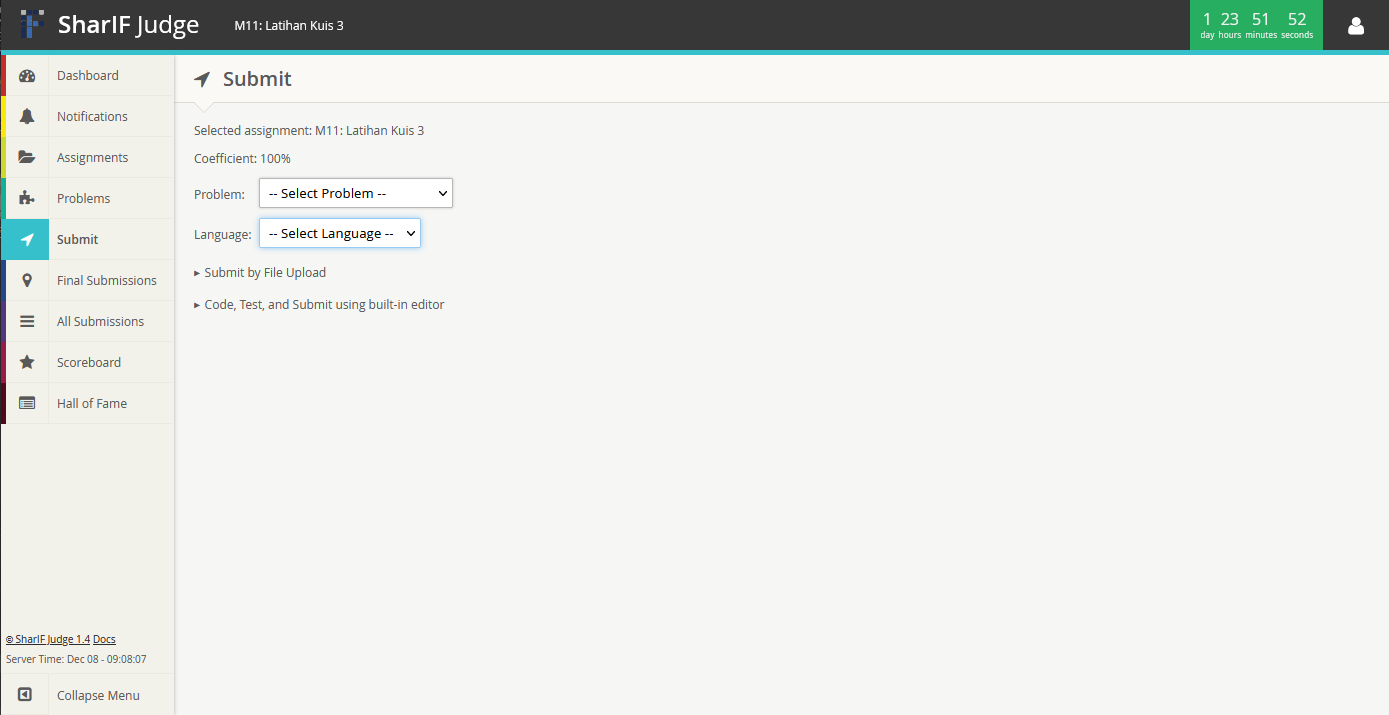
\includegraphics[scale=0.4]{Pengujian/submit_final0.PNG}  
	\caption{Halaman Submit}
	\label{fig:5:submit0} 
\end{figure} 

\begin{figure}[H]
	\centering  
	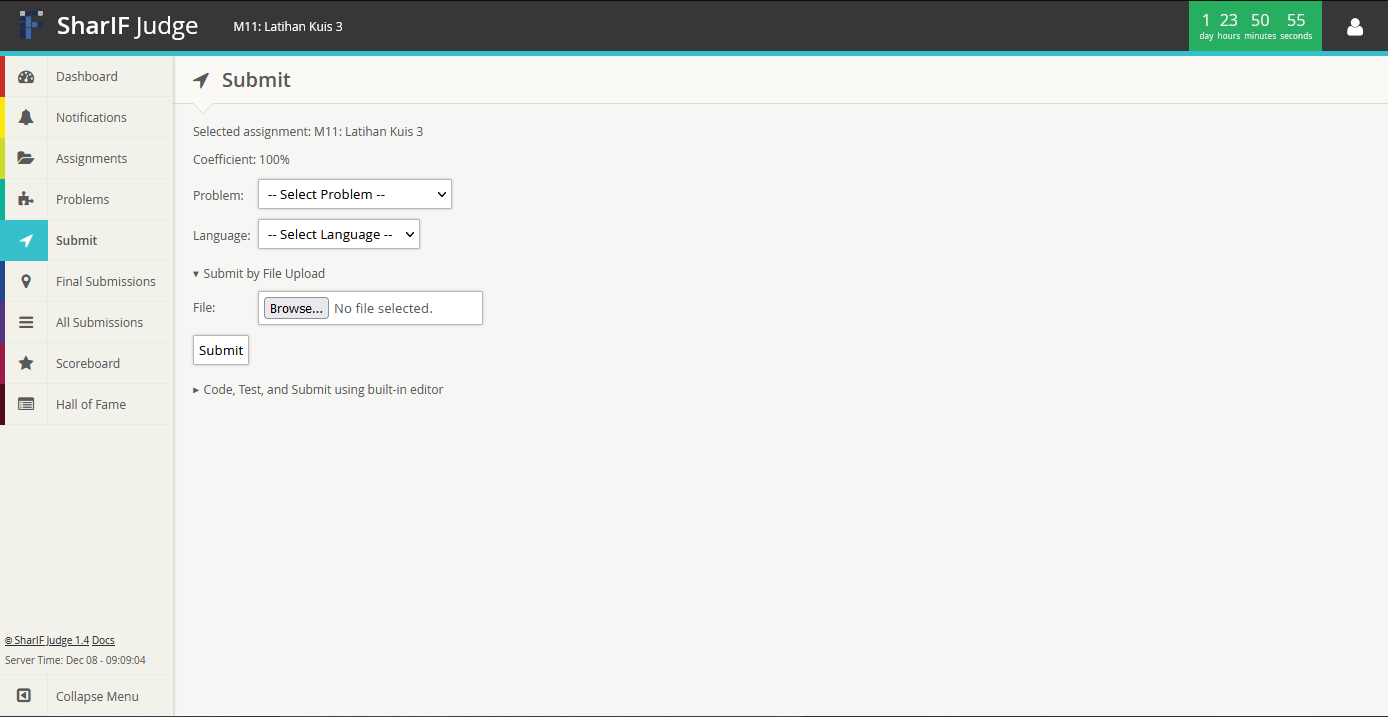
\includegraphics[scale=0.4]{Pengujian/submit_final1.PNG}  
	\caption{Tampilan unggah \textit{file}}
	\label{fig:5:submit1} 
\end{figure} 

\begin{figure}[H]
	\centering  
	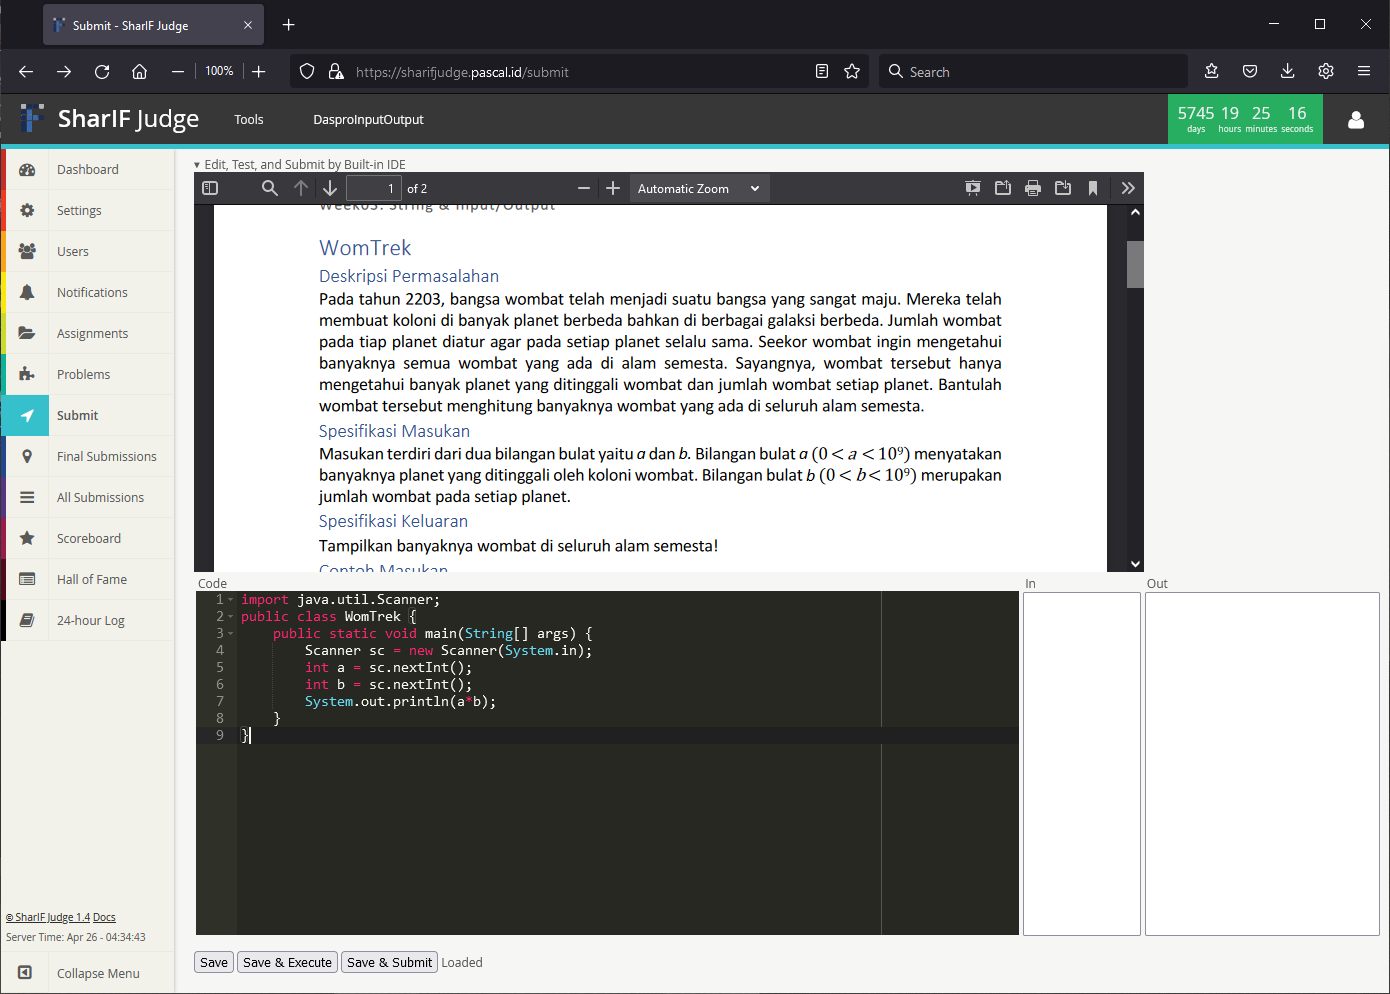
\includegraphics[scale=0.115]{Pengujian/submit_final.PNG}  
	\caption{Tampilan IDE}
	\label{fig:5:submit2} 
\end{figure} 

Gambar \ref{fig:5:submit0} menunjukkan antarmuka halaman Submit setelah perubahan dari masukan ini. Terdapat elemen \textit{summary} pada halaman ini yang dapat ditekan untuk menampilkan antarmuka unggah file seperti pada gambar \ref{fig:5:submit1} dan antarmuka IDE seperti pada gambar \ref{fig:5:submit2}.

\subsubsection{\textit{Submit} Jawaban Soal \textit{Upload Only} Melalui IDE}
Tercatat pada \textit{issue} \#3, ditemukan masalah jika mengumpulkan jawaban untuk soal \textit{upload only}, \textit{status} pada halaman Submissions menjadi "File Not Found".

Masalah ini disebabkan karena variabel \verb|$this->problem['is_upload_only']| pada fungsi \verb|_submit| milik \textit{controller} \verb|Submit| tidak tersedia, sehingga kode dilanjutkan ke dalam antrean untuk dinilai, namun \textit{file} kunci jawaban tidak tersedia, sehingga dikembalikan \textit{status} "File Not Found".

Untuk menyelesaikan masalah ini, dimanfaatkan variabel \verb|$this->problems| yang sudah tersedia pada \textit{controller} \verb|Submit| untuk mengisi variabel \verb|$this->problem['is_upload_only']|. Perubahan ini dapat dilihat pada kode \ref{kode:5:uosubmit} .

\begin{lstlisting}[language=diff, caption=Perubahan pada \texttt{Submit.php}, label=kode:5:uosubmit]
@@ -378,8 +378,15 @@ class Submit extends CI_Controller
                $file_fname = $file_name.'-'.($this->user->selected_assignment['total_submits']+1);
                $file_path = $user_dir.'/'.$file_fname.'.'.$file_ext;

+               foreach($this->problems as $item)
+                       if ($item['id'] == $problem_id)
+                       {
+                               $this->problem = $item;
+                               break;
+                       }
+
                if (!write_file($file_path, $data)){
                       $response = json_encode(array(status=>FALSE, message=>'Unable to submit'));
                }
\end{lstlisting}

\subsubsection{Tidak Bisa \textit{Submit} Melalui Unggah File}
\subsubsection{\textit{Submit} Jawaban txt Melalui IDE}
\subsubsection{Tampilan PDF Viewer jika File PDF Tidak Tersedia}

